\section{Experiments and results}

\begin{figure*}
	\centering
	\subfloat[Control unit]{
	  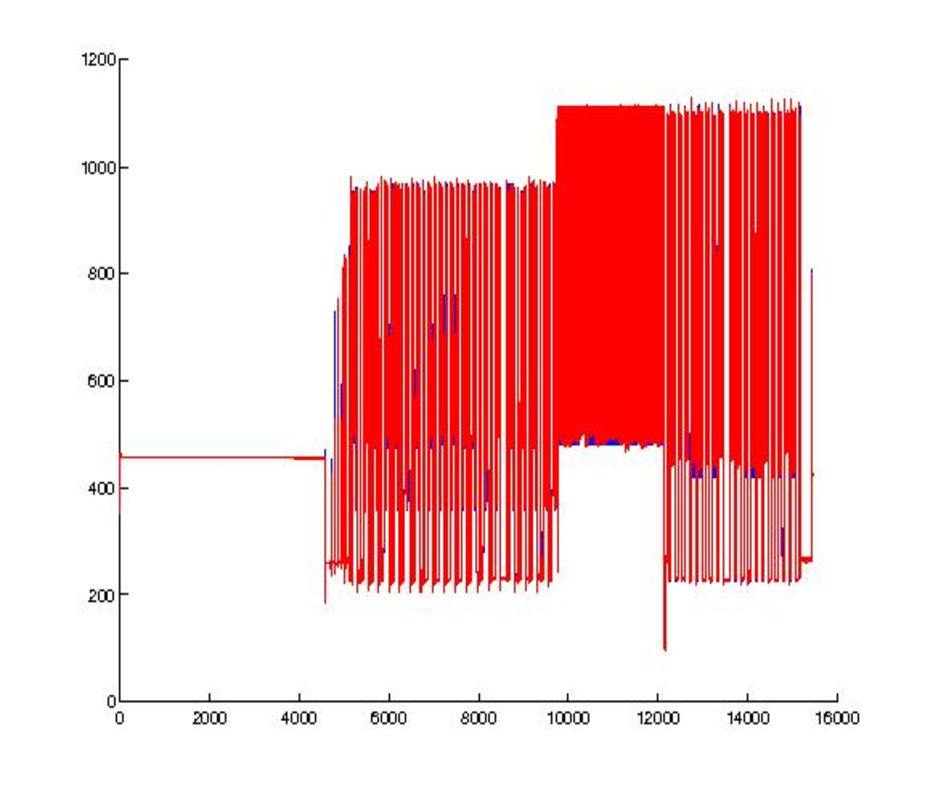
\includegraphics[width=.45\textwidth]{figure/control}
	}
	\subfloat[Data unit]{
	  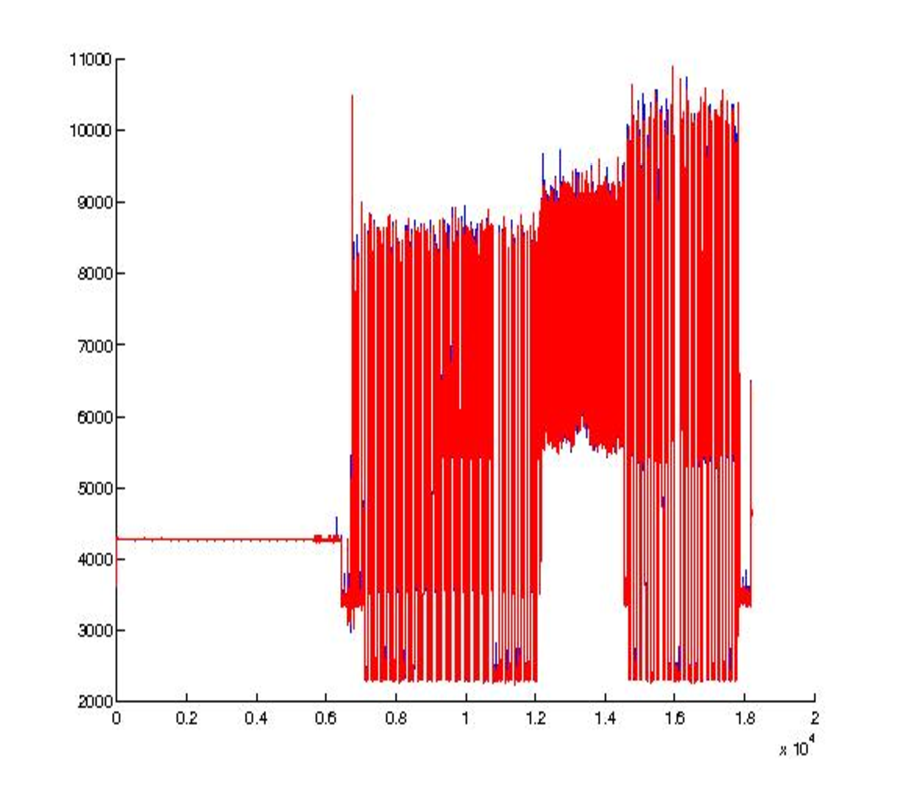
\includegraphics[width=.45\textwidth]{figure/data}
	}
	\\
	\subfloat[Instruction cache]{
	  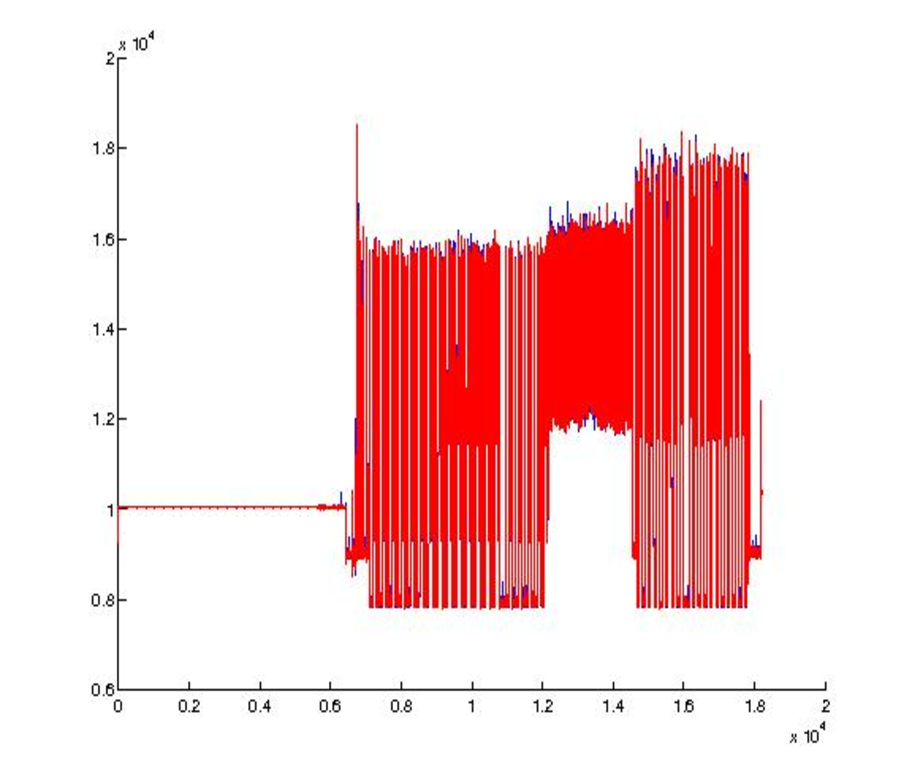
\includegraphics[width=.45\textwidth]{figure/icache}
	}
	\subfloat[Data cache]{
	  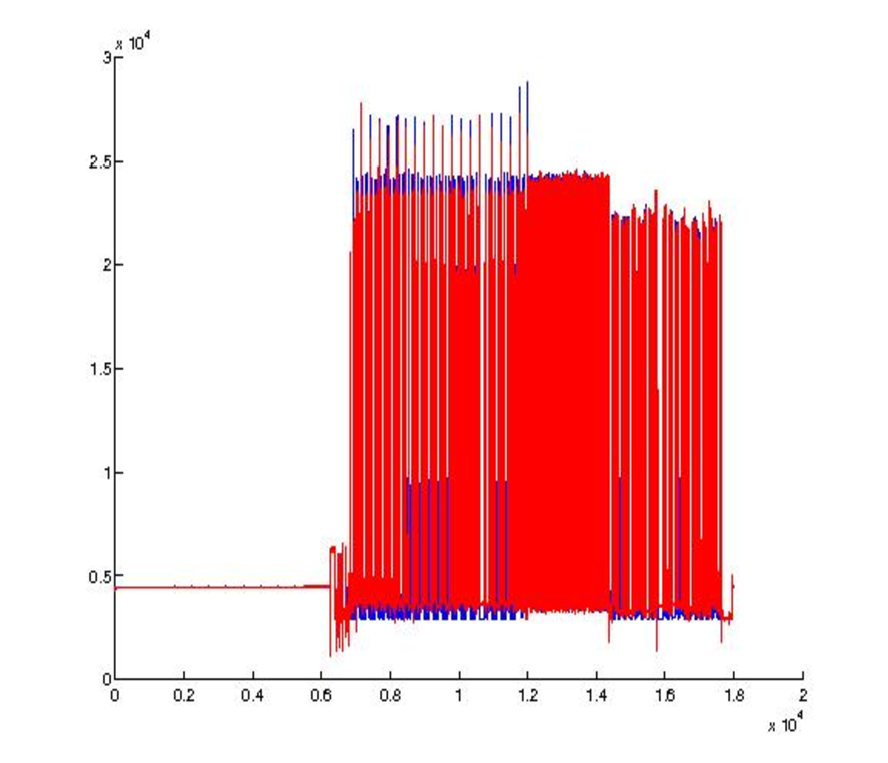
\includegraphics[width=.45\textwidth]{figure/dcache}
	}
	\caption{Comparison between the gate-level power and the linear power model}
	\label{fig:power}
\end{figure*}

Figure \ref{fig:power} shows time-based power analyses for the modules in the RISC-V rocket core.
The red line indicates the gate-level power numbers, and the blue line is the power estimation from the linear power model.
Note that the figures show the linear power model works well for the processors.
